\chapter{Interpolazione}

\section{Teorema}
Se $(x_i, y_i)$, $i=0, \ldots, n$ sono $n+1$ punti distinti, allora esiste un unico polinomio $p_n(x)$ di grado $\leq n$ tale che $p_n(x_i)=y_i$, $i=0, \ldots, n$.




\section{Polinomio interpolatore di Lagrange}

Il polinomio Lagrangiano si presenta nella forma:
\begin{align}
  L_i = \prod_{k=0, k\neq i}^n \frac{x - x_k}{x_i - x_k}
\end{align}

Invece il polinomio interpolatore costruito grazie al polinomio Lagrangiano è:

\begin{align}
  p_n(x) = \sum_{i=0}^n y_i L_i(x)
\end{align}

La caratteristica del polinomio di Lagrange è che:
\begin{align}
  L_i(x_j) = \begin{cases}
    1 & \text{se } i = j \\
    0 & \text{se } i \neq j
  \end{cases}
\end{align}

Il polinomio interpolatore di Lagrange si può riscrivere come:
\begin{align}
  p_n(x)  &= \sum_{i=0}^n y_i L_i(x) \\
          &= \omega_n(x) \sum_{i = 0}^n \frac{\beta_i}{x-x_i}
\end{align}

Dove $\omega_n(x)$ è:
\begin{align}
  \omega_n(x) = \prod_{i=0}^n (x-x_i)
\end{align}


mentre $\beta_i$ è:
\begin{align}
  \beta_i = \frac{y_i}{\prod_{i=0, i\neq j}^n (x_j - x_i)}
\end{align}

Le operazioni necesarie per il calcolo del polinomio interpolatore di Lagrange sono:

\begin{itemize}
  \item $n^2/2$ addizioni
  \item $n^2$ moltiplicazioni
\end{itemize}

Per il calcolo del resto si ricorre alal formula:
\begin{align}
  r(x) &= f(x) - p_n(x) \\
        &= \frac{f^{(n+1)}(\xi)}{(n+1)!} \omega_n(x)
\end{align}


\section{Polinomio di Newton}

Il polinomio di newton(o delle defferenze) si costruisce nel seguente modo, per i $k-1$ punti:

Se $k=0$:
\begin{align}
  f[x_0] &= f(x_0) \\
\end{align}

Se $k=1$:
\begin{align}
  f[x_0,x_1] &= \frac{f[x_1]-f[x_0]}{x_1-x_0} \\
\end{align}

Se $k>1$:
\begin{align}
  f[x_0,x_1,\dots,x_k] &= \frac{f[x_1,x_2,\dots,x_k]-f[x_0,x_1,\dots,x_{k-1}]}{x_k-x_0} \\
\end{align}


Il polinomio finale si costrusce nel seguente modo:
\begin{align}
  f(x) = f[x_0] + (x-x_0)f[x_0,x_1] + (x-x_0)(x-x_1)f[x_0,x_1,x_2] \\ + \dots + (x-x_0)(x-x_1)\dots(x-x_{n-1})f[x_0,x_1,\dots,x_n]
\end{align}



\section{Convergenza dei polinomi di interpolazione}

\subsection{Bernstein}
Se $f(x) \in C^1([a, b])$, il $p_n(x)$ della funzione relativo agli zeri di chebichev di grado $(n+1)$
converge uniformemente a $f(x)$ in $[a, b]$ per $n \rightarrow \infty$.


Se $f(x) \in C^2([a, b])$, l'errore è limitato da:
\begin{align}
  E = O(\frac{1}{\sqrt{n}})
\end{align}

Il polinomio di Bernstein è:
\begin{align}
  B_{n, k}(x) = \binom{n}{k} x^k (1-x)^{n-k}
\end{align}

Dove la binomiale è:
\begin{align}
  \binom{n}{k} = \frac{n!}{k!(n-k)!}
\end{align}





\subsection{Hermite-Fejér}
Sia $f(x) \in C^0([a, b])$, con $[a, b]$ chiuso e limitato e sia:
\begin{itemize}
  \item $p_{2n+1}(x_i) = f(x_i)$
  \item $p'_{2n+1}(x) = 0$
\end{itemize}

Se $x_i$ sono gli zeri di chebichev, allora:
\begin{align}
  \lim_{n \rightarrow \infty} err = 0
\end{align}




\section{Splines}


\subsection{Decomposizione di un intervallo}
Sia $[a, b]$ un'intervallo chiuso e limitato, chiamo decomposizione di $[a, b]$ un insieme finito di punti:

\begin{align}
  \Delta = \{x_0, x_1, \dots, x_n\}
\end{align}



\subsection{Ricerca binaria}
Dato che le spline interpolano gli intervalli, è necessario trovare l'intervallo in cui si trova il punto da interpolare. Per fare ciò si utilizza la ricerca binaria, che permette di trovare l'intervallo in cui si trova il punto da interpolare in $O(\log n)$.

\begin{enumerate}
  \item \textbf{Inizializzazione}: Assicurarsi che l'insieme sia ordinato in modo ascendente.

  \item \textbf{Definire l'intervallo}: Impostare un intervallo di ricerca iniziale che copra l'intero insieme. Solitamente, l'intervallo è definito da due indici: \textit{inizio} e \textit{fine}. All'inizio, \textit{inizio} sarà 0 (indice del primo elemento) e \textit{fine} sarà la lunghezza dell'insieme meno uno (indice dell'ultimo elemento).

  \item \textbf{Calcolare il punto medio}: Calcolare l'indice del punto medio dell'intervallo come \textit{medio = (inizio + fine) / 2}.

  \item \textbf{Confronto}: Confrontare l'elemento nel punto medio con l'elemento cercato.

  \item \textbf{Trova l'elemento}: Se l'elemento nel punto medio è uguale all'elemento cercato, la ricerca è terminata, e l'elemento è stato trovato.

  \item \textbf{Riduzione dell'intervallo}: Se l'elemento nel punto medio è maggiore dell'elemento cercato, impostare \textit{fine = medio - 1} per restringere l'intervallo alla metà inferiore. Altrimenti, se l'elemento nel punto medio è minore dell'elemento cercato, impostare \textit{inizio = medio + 1} per restringere l'intervallo alla metà superiore.

  \item \textbf{Ripeti}: Ripetere i passaggi dal 3 al 6 fino a quando l'elemento viene trovato o finché \textit{inizio} diventa maggiore di \textit{fine}, nel qual caso l'elemento non è presente nell'insieme.
\end{enumerate}



\subsection{Errore della spline}
L'errore della spline è definito come:
\begin{align}
  r(x) &= f(x) - S(x), \quad x \neq x_i \\
       &= | f(x) - S(x) | = \frac{1}{(n+1)!} | f^{(n+1)}(\xi) | \omega(x) \\
       &= \frac{1}{(n+1)!} | f^{(n+1)}(\xi) | \prod_{i=0}^n (x - x_i)
\end{align}





\section{Spline cubica}
Sia $[a, b]$ un intervallo chiuso e limitato, sia $f$ una funzione definita su $[a, b]$ e sia $\Delta = \{x_0, x_1, \dots, x_n\}$ una decomposizione di $[a, b]$. Una spline cubica è una funzione $S$ definita su $[a, b]$ tale che:

\begin{align}
  S_{3, \Delta}(x) = \begin{cases}
    S_{3, \Delta}^1(x) = a^1_0 + a^1_1(x - x_0) + a^1_2(x - x_0)^2 + a^1_3(x - x_0)^3 & x \in [x_0, x_1] \\
    S_{3, \Delta}^2(x) = a^2_0 + a^2_1(x - x_1) + a^2_2(x - x_1)^2 + a^2_3(x - x_1)^3 & x \in [x_1, x_2] \\
    \dotfill \\
    S_{3, \Delta}^n(x) = a^n_0 + a^n_1(x - x_{n-1}) + a^n_2(x - x_{n-1})^2 + a^n_3(x - x_{n-1})^3 & x \in [x_{n-1}, x_{n}]
  \end{cases}
\end{align}


Le incognite sono $a^i_0, a^i_1, a^i_2, a^i_3$ per $i = 1, \dots, n$.
I vincoli sono:
\begin{itemize}
  \item $3(n-1)$ per imporre $C^2([a, b])$
  \item $n+1$ per imporre le interpolazioni ai nodi
\end{itemize}


Ne deriva che vincoli e incognite sono $4n - 2$.

\section{Momenti delle spline}


I momenti delle spline sono definiti come:
\begin{align}
  M_i = [S_{3, \Delta}^i(x_i)]''_{x=x_i}
\end{align}



\subsection{Spline conoscento i momenti}
Se conosco i momenti della spline, posso rappresentare le spline nel seguente modo:
\begin{align}
  S_{3, \Delta}^i(x) = \frac{(x - x_{i-1})^3}{6h_i} M_i + \frac{(x_i -x)^3}{6h_i} M_{i-1} + A_i(x- x_{i-1}) + B_i
\end{align}

Dove:
\begin{align}
  B_i = y_{i-1} - \frac{h_i^2}{6} M_{i-1} \\
  A_i = \frac{y_i - y_{i-1}}{h_i} - \frac{h_i}{6}(M_- - M_{i-1})
\end{align}


Derivando varie volte si ottiene:
\begin{align}
  [S_{3, \Delta}^i(x)]' &= \frac{(x - x_{i-1})^2}{2h_i} M_i - \frac{(x_i -x)^2}{2h_i} M_{i-1} + A_i \\
  [S_{3, \Delta}^i(x)]'' &= \frac{(x - x_{i-1})}{h_i} M_i + \frac{(x_i -x)}{h_i} M_{i-1} \\
  [S_{3, \Delta}^i(x)]''' &= \frac{1}{h_i} M_i - \frac{1}{h_i} M_{i-1}
\end{align}

In tutto questo $h_i = x_i - x_{i-1}$.

\subsection{Convertire momenti in coefficienti}
\begin{align}
  a_0^i &= y_{i-1} \\
  a_1^i &= \frac{y_i - y_{i-1}}{h_i} - \frac{h_i}{6}(2M_{i-1} + M_i) \\
  a_2^i &= \frac{M_{i-1}}{2} \\
  a_3^i &= \frac{M_i - M_{i-1}}{6h_i}
\end{align}


\subsection{Rappresentazione con i momenti}
\begin{align}
  \alpha_i &= \frac{h_i}{h_i + h_{i+1}} \\
  \beta_i &= \frac{h_{i+1}}{h_i + h_{i+1}} \\
  d_i &= \frac{6}{h_i + h_{i+1}} \left( \frac{y_{i+1} - y_i}{h_{i+1}} - \frac{y_i - y_{i-1}}{h_i} \right)
\end{align}

E la rappresentazione diventa:
\begin{align}
  \alpha_i M_{i-1} + 2 M_i + \beta_i M_{i+1} = d_i, \quad i = 1, \dots, n-1
\end{align}

\section{Spline cubica naturale}
Una spline per essere naturale deve avere i momenti $M_0 = M_n = 0$.
Quindi i vincoli diventano:
\begin{align}
  \begin{cases}
    2 M_1 + \beta_1 M_2 = d_1 \\
    \alpha_2 M_1 + 2 M_2 + \beta_2 M_3 = d_2 \\
    \dotfill \\
    \alpha_{n-1} M_{n-2} + 2 M_{n-1} = d_{n-1}
  \end{cases}
\end{align}

La matrice associata è:
\begin{itemize}
  \item triangolare
  \item $\alpha_i + \beta_i = 1$
\end{itemize}


\section{Spline cubica vincolata}
Le condizioni per avere una spline cubica vincolata sono:
\begin{align}
  [S_{3, \Delta}^i(x)]'_{x=x_0} = y_0' \\
  [S_{3, \Delta}^i(x)]'_{x=x_n} = y_n'
\end{align}



La matrice associata è:
\begin{itemize}
  \item tridiagonale
  \item triangolar dominante
  \item irreducibile
\end{itemize}



\section{B\'ezier}

Siano $P_i(x_i, y_i), i = 0, 1, n$, punti di controllo, la curva parametrica si forma:
\begin{align}
  Q_n(t) = \sum_{i=0}^n P_i f_i(t), \quad t \in [0, 1]
\end{align}

$f_i(t)$ sono opportune funzioni polinomiali scelte in modo tale che la curva abbia le seguenti proprietà:

\begin{itemize}
  \item $Q_n(0) = P_0$
  \item $Q_n(1) = P_n$
  \item La tangente in $P_0$ \`e parallela a $P_1 - P_0$
  \item La tangente in $P_n$ \`e parallela a $P_n - P_{n-1}$
\end{itemize}


Queste condizioni sono soddisfate assumendo come funzioni $f_i(t)$ i polinomi di Bernstein:

\begin{align}
  B_i^n(t) = \binom{n}{i} t^i (1-t)^{n-i}, \quad i = 0, 1, n
\end{align}

Dove la binomiale si calcola come:
\begin{align}
  \binom{n}{i} = \frac{n!}{i!(n-i)!}
\end{align}


Quindi la curva di B\'ezier \`e data da:
\begin{align}
  Q_n(t) = \sum_{i=0}^n P_i B_i^n(t), \quad t \in [0, 1]
\end{align}

\begin{figure}[h!]
  \centering
  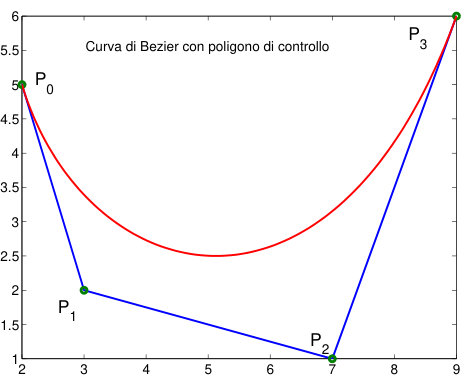
\includegraphics[width=0.4\linewidth]{images/curva_bazier_esempio.png}
\end{figure}



Spesso \`e necessario utilizzare pi\`u curve e per fare ci\`o si utilizzano i gradi di continuith\`a.

\begin{itemize}
  \item $C^0$, le due curve hanno un punto in comune (primo nodo della seconda curva coincide con l'ultimo della prima)
  \item $C^1$, le due curve hanno un punto in comune e la derivata prima \`e uguale in direzione e modulo
\end{itemize}

\subsection{Curve di B\'ezier razionali}

In questo caso si introduce un valore di peso per ogni punto di controllo, quindi la curva \`e data da:
\begin{align}
  Q_n(t) = \frac{\sum_{i=0}^n P_i w_i B_i^n(t)}{\sum_{i=0}^n w_i B_i^n(t)}, \quad t \in [0, 1]
\end{align}


\begin{figure}[h!]
  \centering
  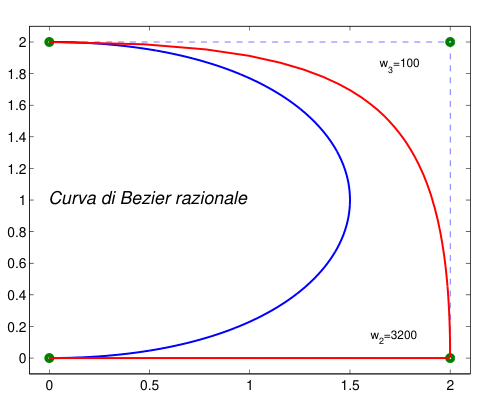
\includegraphics[width=0.4\linewidth]{images/bazier_pesato_esempio.png}
\end{figure}



\section{Interpolazione di funzioni in pi\`u variabili}
Sapendo che il polinomio Lagrangiano \`e:
\begin{align}
  L_{ij}(x, y) = L_i(x) L_j(y)
\end{align}

Il polinomio interpolante \`e:
\begin{align}
  p_{n, m}(x, y) &= \sum_{i=0}^n \sum_{j=0}^m f(x_i, y_j) L_{ij}(x, y) \\
  &= \sum_{i=0}^n \sum_{j=0}^m f(x_i, y_j) L_i(x) L_j(y)
\end{align}
